\subsection{Client-side Middleware}

%As described in Section~\ref{sec:proposal}, the CSM component interacts with DSM from different domains that could be either discoverable using a DNS-like mechanism or advertisement. 

The goal of the client-side middleware is to allow client applications to invoke A3-E microservices without knowing where they will actually be executed within the computing continuum: locally on the mobile device, in a local-edge server, in a mobile-edge server, or in the cloud. 

Its selection algorithm is a multi-objective function that takes into account the requirements of the functions and the availability of the various domains. 

The implementation we present\footnote{Documentation and source code are available at \url{https://github.com/deib-polimi/A3-E-CSM}} is in Java, so that it could be run on Android-based evices. However, it does not use Android-specific technology and can therefore easily be generalized to any client platform. 

\begin{figure}[tbp]
	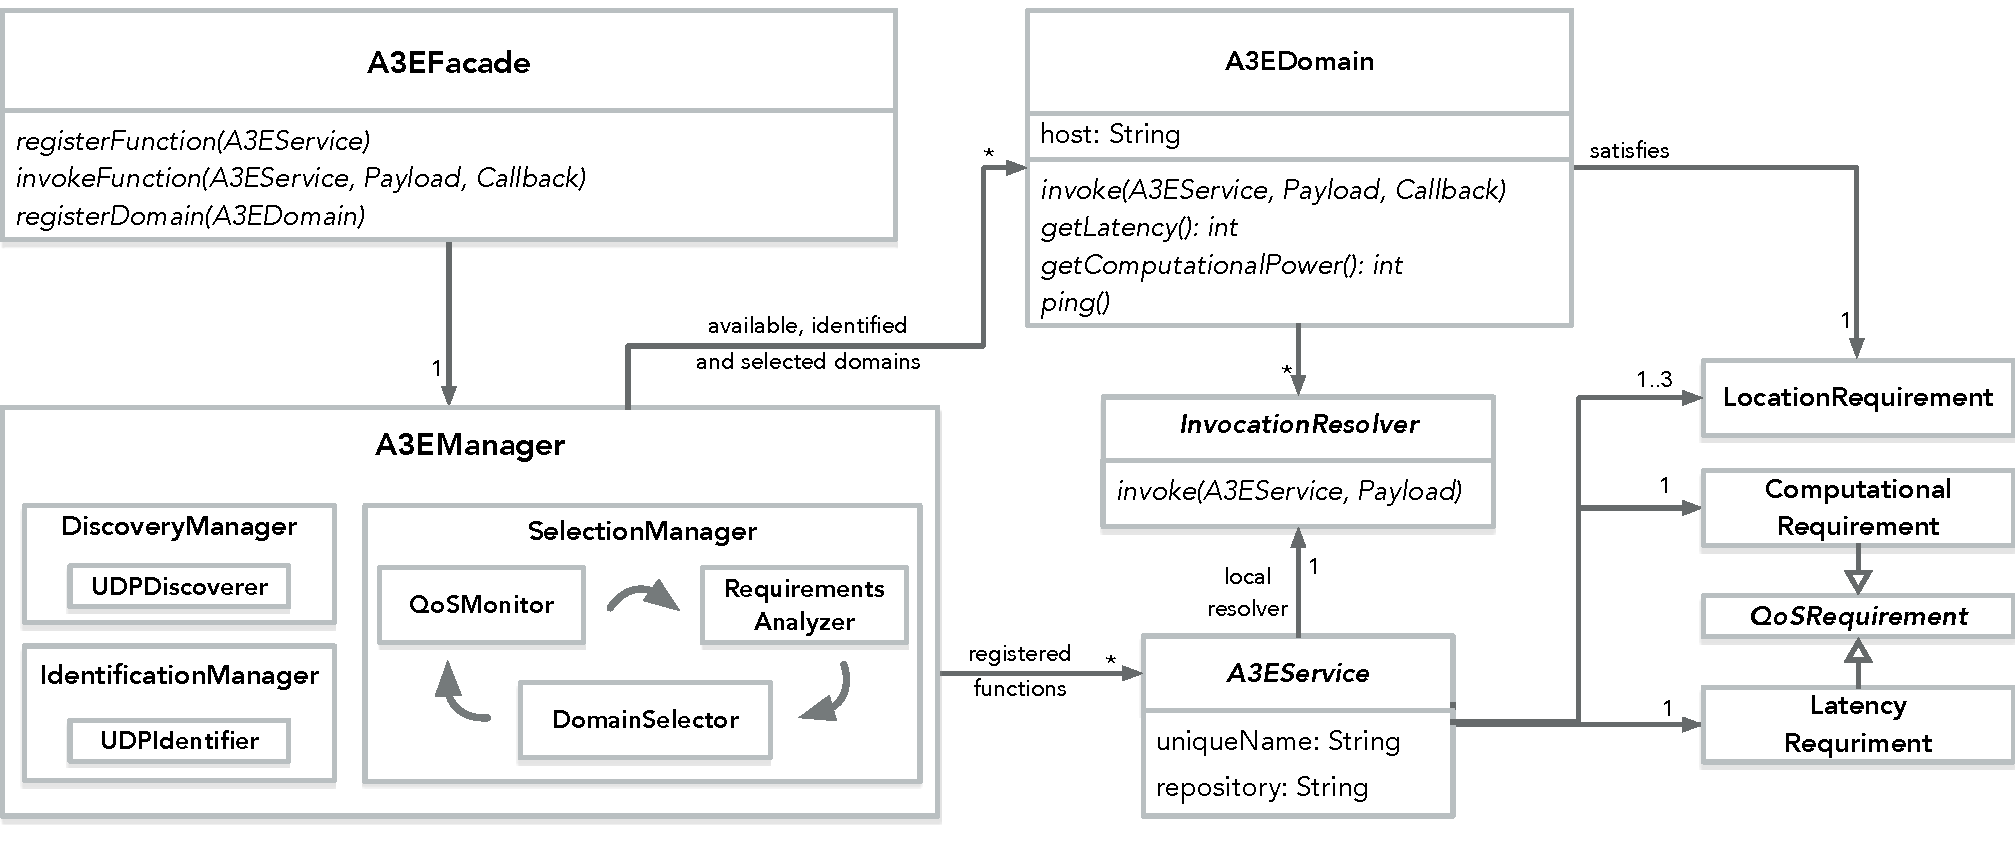
\includegraphics[width=1\textwidth]{figs/a3e-mobile-prototype}
	\caption{Client-side Middleware Architecture}
	\label{fig:mobile-prototype}
\end{figure}

Figure~\ref{fig:mobile-prototype} shows the high-level architecture of the client-side middleware. Client mobile applications interact with two components: \textit{A3EFunction}s and \textit{A3EFacade}. The former abstracts the actual functions to be executed, while the latter is used to register and execute functions. 

An \textit{A3EFunction} is identified by a unique name, the url of its git coede repository, and declares three types of QoS requirements: 
%that corresponds to the name of the function asset that must be communicated to the continuum domains to be first acquired and then executed. Moreover each function must declare a set of non-functional QoS requirements that are organized in three types: 

\begin{enumerate}

	\item a \textit{Location Requirement} constrains where the function will be placed within the continuum, i.e., \textit{LOCAL}, \textit{LOCAL-EDGE}, \textit{MOBILE\_EDGE}, and \textit{CLOUD}; 

	\item a \textit{Latency Requirement} constrains network latency, i.e., \textit{ANY}, \textit{LOW} or \textit{VERY LOW}; and 
	
	\item a \textit{Computational Requirement} defines how relevant it is for a function to have fast computing, i.e., \textit{ANY}, \textit{FAST} or \textit{VERY FAST}. 

\end{enumerate}

%Before becoming able for execution, the function must be registered using the \textit{A3EFacade}. 

%\begin{itemize}
	%\item \textit{Location Requirement}s are constrains over the continuum. A function can declare where it could be executed choosing a combination of three values: \textit{LOCAL}, \textit{EDGE} and \textit{CLOUD}. By default an \textit{A3EFunction} supports all three domain types but one can implement a function that, for example, cannot be executed locally thus only the \textit{EDGE} and \textit{CLOUD} requirements should be added.    
	%\item \textit{Latency Requirement} expresses how important for a function is to have a low networking latency. The default value is \textit{LOW} since the main motivation of the work is to support low-latency applications. An \textit{A3EFunction}  can  also state that this requirement should be \textit{ANY} or \textit{VERY LOW}. The lower the latency requested the more the networking latency will be considered important in the the domain selection procedure.
	%\item \textit{Computational Requirement} defines how relevant for a function is to have a fast computing processing. The predefined value is \textit{FAST}, since, again, the main targets of the approach are applications that requires fast request/response interactions. Similarly to the latency requirement two additional values are available:  \textit{ANY} or \textit{VERY FAST}. The higher  processing power is requested the more this metric will be considered important during the domain selection phase.
%\end{itemize}

%An \textit{A3EFunction} that support the \textit{LOCAL} location requirement should also define a local \textit{InvocationResolver}. As we are going to discuss later in this section, invocation resolvers deal with the invocation technology \textit{heterogenity}  of the continuum. For what regards the local domain we currently support the execution of native Java code and Javascript functions (that could be imported in the project as standard \textit{.js} files). For this purpose we created two \textit{InvocationResolver}s that can execute respectively Java or Javascript functions if the local domain is selected.

The \textit{A3EFacade} component wraps the \textit{A3ELoopManager}, which manages all the registered \textit{A3EFunctions}. It consists of a MAPE control loop~\cite{kephart2003vision} for the discovery, identification and selection of domains, corresponding to the \textit{Awareness}, \textit{Acquisition}, and \textit{Allocation} phases of the A3-E model. 

%The loop manager  consists of three main components called \textit{DiscoveryManager}, \textit{IdentificationManager} and \textit{SelectionManager}. 

Component \textit{DiscoveryManager} manages the discovery of domains. The local domain is registered when the middleware is created, while cloud domains are registered by the client application and their endpoints must be known a-priori. Edge domains, on the other hand, are found at run time. Every time the IP address of the client device changes, the manager starts listening for UDP broadcast message. If a message is received, the IP address of the sender is retrieved and a new \textit{A3EDomain} is created in the middleware. An \textit{A3EDomain} is identified by a \textit{host} name (URI) and satisfies a specific \textit{LocationRequirement}. Component \textit{InvocationResolver} is then used to actually invoke the microservices. 
%An  \textit{A3EDomain} could be either \textit{static} or \textit{dynamic}. Static domains are added to the discovery manager at launch time, meaning that it is known a-priori that they will be available. Example of this are cloud and local domains. On contrary dynamic domains can be found only at runtime with appropriate technological protocols (such as DNS and advertising). Edge domains are not known a-priori thus they are considered dynamic. Static domains can be added by the client application using the \textit{registerDomain} operation provided by the \textit{A3EFacade} while dynamic domains are automatically discovered by the \textit{DiscoveryManager}.
 %\textit{A3EDomain}s  are identified by a \textit{host} name, that is a unique network identifier by which it is possible to interact with the domain using a network. Moreover, as shown in the figure, a domain is considered \textit{Pingable} that means that it is possible to check for its availability and measure its networking latency (in milliseconds). Each domain satisfy a \textit{LocationRequirement}, intuitively local domains satisfies the \textit{LOCAL} requirement, while the edge and cloud ones the \textit{EDGE} and \textit{CLOUD} respectively.  A domain also provides three additional operations: one to execute a function within the domain, one to retrieve the networking latency (its value is lazily updated after a \textit{ping}) and one to obtain its computational power. Finally a domain also uses an \textit{InvocationResolver} to actually invoke the function. 
In addition to finding new domains, the \textit{DiscoveryManager} also checks for their availability. Once every control loop iteration, existing domains are pinged to calculate their network latency. After that, the \textit{IdentificationManager} is activated.

%The output of this process is the list of the available domains. 
 %This component initializes the identification phase for each new available domain (e.g., domains discovered for the first time). 

The \textit{IdentificationManager} checks which registered A3-E functions can be executed on each domain, according to their location requirements. It then requests those functions (eventually triggering the allocation phase in the domain), and finally retrieves the domain's computational power --- a fixed score ranging from $1$ to $5$\footnote{Labeling computational power is also common in the cloud where different tiers of virtual machines are available -- \url{https://aws.amazon.com/ec2/instance-types/}}. %where the local domain is set to $1$, the edge domains to $4$ and the cloud ones to $5$. 
Note that since the cloud provides the illusion of infinite scalability it gets the maximum score, regardless of the VMs that are actually being used. More sophisticated approaches, such as using dynamic scores that change according to the saturation of the domain, or to the battery level, are considered future work.  

\begin{algorithm}[b]
	\caption{A3E Selection Algorithm}
	\label{alg:selection}
	\begin{algorithmic}[1]
		
		\Function{selectDomain}{A3EFunction $function$, A3EDomain[] $identifiedDomains$}
		\State$scoreRange \gets 5$
		\State $maxLatency \gets \Call{computeMaximumLatency}{identifiedDomains}$
		\State $maxCpuPower \gets \Call{computeMaximumComputationalPower}{identifiedDomains}$
		\State $latencyWeight \gets function.getLatencyRequirement()$ 
		\State $cpuPowerWeight \gets function.getComputationalPowerRequirement()$ 
		\State $maxScore \gets 0$
		\State $selectedDomain \gets null$
		\ForAll{$domain \in identifiedDomains$ } 
		\State $latency \gets domain.getLatency()$ 
		\State $cpuPower \gets function.getComputationalPower()$ 
		\State $latencyScore \gets latencyWeight*((scoreRange-1)*(1 - latency/maxLatency)+1)$ 
		\State $cpuPowerScore \gets cpuPowerWeight*(scoreRange*(cpuPower/maxCpuPower))$
		\State $score \gets (latencyScore + cpuPowerScore) / (latencyWeight + cpuPowerWeight)$
		\If{$score \geq maxScore$} 
		\State $maxScore \gets score$
		\State $selectedDomain \gets domain$
		\EndIf
		\EndFor 
		\State \Return $selectedDomain$
		\EndFunction
	\end{algorithmic}
\end{algorithm}

At the end of the identification phase, the network latency and computational power of each domain is known, and the domains are considered ready to execute functions (i.e., proactive approach). At this point component \textit{SelectionManager} starts the selection process as described in Algorithm~\ref{alg:selection}. 

%The procedure is activated for each registered function with the identified domains (line $1$). The algorithm computes a score ranging from $0$ to $5$ (line $2$) for each domain and selects the highest one. The current implementation considers as quality metrics the networking latency and the computational power. The first step of the selection consists on computing the maximum latency and computational power (line $3$ and $4$) among the identified domains. This data, as already mentioned, were gathered during the previous phases. Then the weights of latency and computational power are retrieved (lines $5$ and $6$). These weights correspond to the values associated to the \textit{LatencyRequirement} and \textit{ComputationalPowerRequirement} of the function. The \textit{ANY} value corresponds to a weight of $0$, a latency requirement of \textit{LOW} and a computational power requirement of \textit{FAST} correspond to a weight equal to $1$, while weight equals to $2$ is considered for both latency \textit{VERY LOW} and computational power \textit{VERY FAST}.

%For each domain, the algorithm computes the overall score (line  $9$ to $14$). The latency score is computed by normalizing the value retrieved at line $10$ with the maximum latency previously computed. The normalized value ranges from $0$ to $1$, the higher this value the higher the latency. Since a higher score should mean lower latencies, the algorithm computes the complement of this value and add $1$ to avoid scores equals to $0$. Finally, the latency score is computed to be in the range of $5$ and multiplied by the function's latency weight (line $12$). The computational power score is computed by normalizing the domain computational power retrieved at line $11$ with the  maximum value across the identified domains. Then the score for this metric is computed to be in the range of $5$ and multiplied by its weight (line $13$). Finally the overall score is computed by performing a weighted average between the scores obtained by the domains for the two QoS metrics.

%Two considerations must be added for this algorithm. First, 
The procedure it follows is an instantiation of the SMART decision process~\cite{Olson1996}, in which multiple competing QoS objectives are considered using the following formula

\begin{equation}
Smart(c) = \frac{\sum_{i=1}^{n} QoSAtrribute_i(c)*weight_i}{\sum_{i=1}^{n}weight_i} \label{eq:smart}
\end{equation}

where, in the context of our approach, $c$ is a domain, the QoS attributes values are network latency and the computational processing time (thus $n$ is $2$), and their weights are represented by the aforementioned latency and computation requirements. Note that, when available, \textit{edge domains have the highest chances of being selected}, since they usually combine a low network latency and a medium-to-high computational power. Finally, each function is mapped to the domain that best satisfies its requirements. 

At a customizable control interval (the default is set to $2$ seconds) the control loop starts looking for new domains, recalculates the domains' network latencies and potentialy  improves the selection.

During \textit{Engagement} phase the actual function execution takes place. The client application can execute a function using the \textit{execute} operation of the  \textit{A3EFacade}. %In addition to the \textit{A3EFunction}, the operation expects also a \textit{payload} (i.e., the function argument) that could be an object of any Java type, and a \textit{callback} since the execution is always asynchronous. 
The \textit{A3EFacade} will retrieve the \textit{A3EDomain} that was selected for the function in the last control loop iteration. Since domains use heterogeneous technologies, the actual executions are perfromed by the \textit{InvocationResolver} components that are bound to different domains. Asynchronous \textit{callback}s are used to provide the results back to the client applications. %\textit{InvocationResolver}s hide the technological details of the underlying domains. 


% bound to the domain will be used to actually \textit{execute} the function.  
%Since the control loop runs in a separated thread, the execution will not be affected if the selected domain changes during the invocation. After retrieving the best domain from the continuum, the \textit{A3EFacade} will execute the function by using the \textit{execute} operation of the \textit{A3EDomain}. Since each domains can use different technologies, the \textit{InvocationResolver} binded to the domain will be used to actually invoke the function. 

%addressing the \textit{heterogeneity} property of the continuum. 
In our current implementation of the client-side middleware we have four types of \textit{InvocationResolver}s: two for executing functions that are deployed inside the actual mobile device (one written in Javascript and one in Java), one for Rest HTTP calls (to support multiple FaaS platforms such as OpenWhisk\footnote{\url{https://github.com/apache/incubator-openwhisk/blob/master/docs/webactions.md}}), and one specifically for AWS Lambda\footnote{\url{https://aws.amazon.com/tools/\#sdk}}. %and finally a local invocation resolver that is binded to the local domain that simply forward the invocation to the function's local \textit{InvocationResolver} (either the \textit{JavaInvocationResolver} or \textit{JSInvocationResolver}).  


%Since each function has its own characteristics, for example different REST calls could have different \textit{content-type}s and different format for input/output, we made each function able to modify the invocation with it is own applicative details. For this reason before invoking the actual function (e.g., performing the HTTP call) the \textit{InvocationResolver} creates a technology specific \textit{InvocationMean}. These components are wrappers to technology specific objects used by the invocation resolvers to build the call (e.g., the \textit{InvokeRequest\footnote{\url{http://docs.aws.amazon.com/AWSJavaSDK/latest/javadoc/com/amazonaws/services/lambda/model/InvokeRequest.html}}} object of the AWS Lambda SDK). As shown in Figure~\ref{fig:mobile-prototype} \textit{A3EFunction}s are \textit{InvocationMeanVisitor}s. Thus, just before performing the invocation, the specific \textit{visit} method is call providing to the function a way to fill up the request for the specific type of call. 

%To summarize, supporting the continuum with A3E in a client application consists in the following four steps\footnote{A simple example of use can be found at \url{https://github.com/gioenn/a3e-android/blob/master/README.md}}:

%\begin{enumerate}
%	\item Register static \textit{A3EDomain}s such as cloud endpoints.
%	\item Create \textit{A3EFunction}s and override the specific methods to customize the requests for the technologies of interest
%	\item Register the functions
%	\item Execute the functions in the continuum as plain programmatic calls 
%\end{enumerate}